\subsection{Tipos de servidores}
\label{section:tipos_de_servidores}
\paragraph{}
Guardadas as devidas configura\c{c}\~oes f\'isicas, tipos de mem\'oria, cpu ,entre outros, h\'a dois poss\'iveis tipos de servidores:  Servidor de origem e servidor de ponta.

\paragraph{Servidores de origem}s\~ao servidores onde toda a informa\c{c}\~ao vai ficar baseada. \'E o lugar onde v\~ao ser armazenados os conte\'udos e o ponto principal do sistema.
\paragraph{}
\'E ele o respons\'avel por, na aus\^encia da informa\c{c}\~ao perto do cliente, fornecer tudo o que o cliente necessita de informa\c{c}\~ao. E em caso de um primeiro acesso \'e atrav\'es dele que ser\'a feito o interfaceamento entre usu\'ario e conte\'udo.
\paragraph{}
H\'a uma necessidade intr\'inseca de que esse servidor tenha excelentes configura\c{c}\~oes f\'isicas e \'otimas regras de seguran\c{c}as, \textit{firewall} incluso, que possam garantir a integridade do sistema mesmo em caso de muitos acessos.
\paragraph{Servidores de ponta}s\~ao servidores que mais pr\'oximos aos clientes. Parte do conte\'udo do servidor de origem estar\'a replicado nele. Dizemos em parte, pois n\~ao sabemos quais pol\'iticas de \textit{cache} que ser\'a adotada pelos criadores da rede. 
\\
Podemos ilustr\'a-los conforme a figura \ref{figura:tipos_servidores}.
\begin{figure}[H]
\caption{Tipos de servidores}
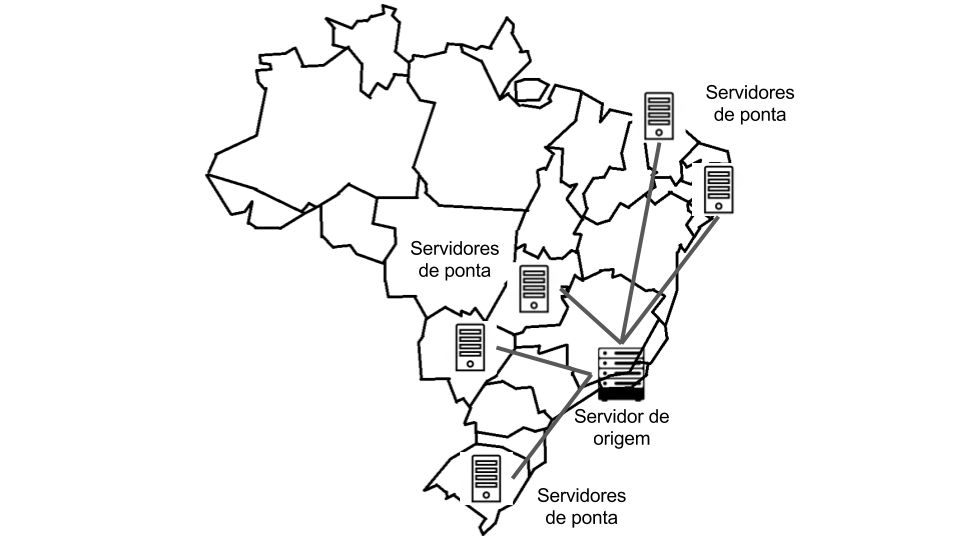
\includegraphics[height=9cm]{Figuras/tipos_servidores.png} 
\label{figura:tipos_servidores} 
\end{figure}

Vale salientar que n\~ao necessariamente esses \textit{status} de ser de ponta ou ser de origem s\~ao imut\'aveis. Em ambientes reais e comerciais um servidor de origem \'e tamb\'em um servidor de ponta para um outro conte\'udo. Isso \'e o respons\'avel por tornar as grandes cdns completamente transparentes geograficamente perante aos seus clientes.